\subsection{CR Alternativi: CTFBox}\label{cr-alternativi-ctfbox}

CTFBox e\textquotesingle{} un Cyber Range perfetto per organizzare CTF
di tipo Attack/Defense, dove ogni team ha una macchina con uno o piu
servizi vulnerabili da difendere, mentre si attaccano i servizi esposti
sulle macchine avversarie per recuperare le flag. Durante il gioco, ogni
team deve fare attenzione a non rompere i propri servizi, mantenendo
un\textquotesingle alta percentuale di SLA. Una SLA bassa comporta una
penalita\textquotesingle{} in termini di punteggio. \footnote{\label{fn:ref_9}\url{https://ctfbox.domy.sh/}}

Fa uso di \textbf{Docker} per gestire i servizi essenziali del gioco (e
che costituiscono quindi CTFBox), mentre \textbf{Incus} viene utilizzato
per gestire l\textquotesingle esecuzione delle macchine virtuali o dei
container dei team.


\begin{figure}[htbp]
  \centering
  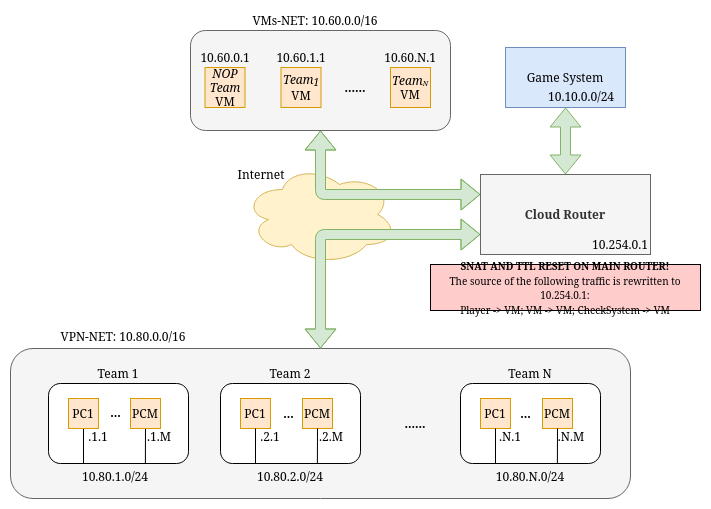
\includegraphics[width=0.85\linewidth,height=0.65\textheight,keepaspectratio]{src/images/ctfbox-architecture.png}
  \caption{Ctfbox Architecture}
  \label{fig:ctfbox-architecture}
\end{figure}


\textbf{Router}: e\textquotesingle{} un container Docker, che gestisce
le configurazioni della rete WireGuard, permettendo ai giocatori di
connettersi alla rete di gioco. Controlla le regole di routing sulla
rete, e governa la transizione della rete tra 3 stati diversi:

\begin{itemize}
\tightlist
\item
  \passthrough{\lstinline!freeze!}: in questo stato, nessuno
  puo\textquotesingle{} accedere alle macchine vulnerabili
\item
  \passthrough{\lstinline!lock!}: in questo stato, ogni team
  puo\textquotesingle{} accedere solo alla propria macchina vulnerabile.
\item
  \passthrough{\lstinline!unlock!}: in questo stato, la rete
  e\textquotesingle{} completamente aperta, i team possono attaccare le
  macchine avversarie.
\end{itemize}

\textbf{Game System}: e\textquotesingle{} un container Docker, che
agisce da cervello centrale per la gestione del gioco.

\begin{itemize}
\tightlist
\item
  Gestisce lo stato della rete (freeze/lock/unlock), comunicando i
  cambiamenti al router.
\item
  Mantiene il database delle flag, e calcola i punteggi per ogni team.
\item
  Coordina i Checkers, ossia i worker che interrogano i servizi dei team
  ad ogni tick.
\end{itemize}

In CTFBox, ad ogni tick (ossia ogni round di gioco), le flag vengono
rigenerate su ogni macchina, per ogni servizio vulnerabile, e registrate
nel database. L\textquotesingle obiettivo di un team in una competizione
Attack/Defense strutturata in questo modo e\textquotesingle{} di
attaccare piu volte lo stesso servizio sulle macchine avversarie, per
recuperare quante piu flag possibli, finche le difese avversarie non
bloccano gli attacchi.

\textbf{Checkers}, ad ogni tick (o round) fanno due cose:

\begin{enumerate}
\def\labelenumi{\arabic{enumi}.}
\tightlist
\item
  Interrogano tutti i servizi vulnerabili attivi, e determinano la
  percentuale di SLA per ogni team.
\item
  Installano le nuove flag sui servizi vulnerabili.
\end{enumerate}

Ogni membro del team, ha la sua configurazione \textbf{WireGuard} per
conettersi alla propria macchina e per raggiungere le macchine
avversarie. Ad ogni giocatore che si connette viene assegnato
un\textquotesingle indirizzo nella sottorete
\passthrough{\lstinline!10.80.team\_id.0/24!} mentre le macchine dei
team si trovano nella sottorete \passthrough{\lstinline!10.60.0.0/16!}.

Dunque CTFBox si rileva essere un\textquotesingle ottimo sistema per
gestire competizioni Attack/Defense e per regolare
l\textquotesingle accesso alle macchine, ma la sua architettura non si
applica in contesti in cui vorremmo solo assegnare ad ogni team un
insieme di macchine vulnerabili il cui stato verra\textquotesingle{} poi
verificato da un\textquotesingle oracolo.
